\documentclass[
	% -- opções da classe memoir --
	12pt,				% tamanho da fonte
	openright,			% capítulos começam em pág ímpar (insere página vazia caso preciso)
	oneside,			% para impressão em apenas anverso. Oposto a twoside
	%twoside,			% para impressão em verso e anverso. Oposto a oneside
	a4paper,			% tamanho do papel. 
	% -- opções da classe abntex2 --
	%chapter=TITLE,		% títulos de capítulos convertidos em letras maiúsculas
	%section=TITLE,		% títulos de seções convertidos em letras maiúsculas
	%subsection=TITLE,	% títulos de subseções convertidos em letras maiúsculas
	%subsubsection=TITLE,% títulos de subsubseções convertidos em letras maiúsculas
	% -- opções do pacote babel --
	english,			% idioma adicional para hifenização
	brazil				% o último idioma é o principal do documento
]{abntex2}

% Evita linhas orfãs e viúvas
\widowpenalty=10000
\clubpenalty=10000

\usepackage{lmodern}			% Usa a fonte Latin Modern
\usepackage[T1]{fontenc}		% Selecao de codigos de fonte.
\usepackage[utf8]{inputenc}		% Codificacao do documento (conversão automática dos acentos)
\usepackage{lastpage}			% Usado pela Ficha catalográfica
\usepackage{indentfirst}		% Indenta o primeiro parágrafo de cada seção.
\usepackage{color}				% Controle das cores
\usepackage{graphicx}			% Inclusão de gráficos
\usepackage{microtype} 			% para melhorias de justificação
\usepackage{lipsum}				% para geração de dummy text
\usepackage[alf]{abntex2cite}					% Citações padrão ABNT
\usepackage{tikz}
\usetikzlibrary{shapes,arrows,chains}
\usepackage[]{mcode}
\usepackage{multirow}
\usepackage{array}
\usepackage{longtable}
\usepackage{rotating}
\usepackage{caption}
\usepackage{pbox}
\usepackage{pdfpages}
\usepackage{float}
\usepackage{amsmath}

\usepackage{todonotes}

\graphicspath{{../Mathematica}{../Mathematica/Images}}

\usepackage[brazil]{babel}		% idiomas
\addto\captionsbrazil{
	%% ajusta nomes padroes do babel
	\renewcommand{\bibname}{Refer\^encias Bibliogr\'aficas}
	\renewcommand{\indexname}{\'Indice Remissivo}
	\renewcommand{\listfigurename}{Lista de Figuras}
	\renewcommand{\listtablename}{Lista de Tabelas}
	\renewcommand{\listadesiglasname}{Lista de Abreviaturas e Siglas}
	%% ajusta nomes usados com a macro \autoref
	\renewcommand{\pageautorefname}{p\'agina}
	\renewcommand{\sectionautorefname}{se{\c c}\~ao}
	\renewcommand{\subsectionautorefname}{subse{\c c}\~ao}
	\renewcommand{\paragraphautorefname}{par\'agrafo}
	\renewcommand{\subsubsectionautorefname}{subse{\c c}\~ao}
}


\definecolor{blue}{RGB}{0,114,189}
\definecolor{orange}{RGB}{217,83,25}
\definecolor{yellow}{RGB}{237,177,32}
\definecolor{purple}{RGB}{126,47,142}
\definecolor{green}{RGB}{119,172,48}
\definecolor{lightBlue}{RGB}{77,190,238}
\definecolor{red}{RGB}{162,20,47}
\definecolor{black}{RGB}{0,0,0}

% informações do PDF
\makeatletter
\hypersetup{
     	%pagebackref=true,
		pdftitle={\@title}, 
		pdfauthor={\@author},
    	pdfsubject={\imprimirpreambulo},
	    pdfcreator={LaTeX},
		pdfkeywords={abnt}{latex}{abntex}{abntex2}{trabalho acadêmico}, 
		colorlinks=true,	% false: boxed links; true: colored links
    	linkcolor=black,	% color of internal links
    	citecolor=black,	% color of links to bibliography
    	filecolor=black,	% color of file links
		urlcolor=black,
		bookmarksdepth=4
}
\makeatother

% --- 
% Espaçamentos entre linhas e parágrafos 
% --- 
% O tamanho do parágrafo é dado por:
\setlength{\parindent}{1.3cm}
% Controle do espaçamento entre um parágrafo e outro:
\setlength{\parskip}{0.2cm}  % tente também \onelineskip



\titulo{Método de classificação de build orders em StarCraft II}
\autor
{
	UNIVERSIDADE FEDERAL DO RIO GRANDE DO SUL\\
	ESCOLA DE ENGENHARIA\\
	DEPARTAMENTO DE ENGENHARIA ELÉTRICA\\
	\vspace*{4\baselineskip} 
	ROGIEL JOSIAS SULZBACH
}
\local{Porto Alegre}
\data{2016}
\orientador{Prof. Dr. Altamiro Amadeu Susin}
\coorientador{}
\instituicao{}
\preambulo{Projeto de Diplomação apresentado ao Departamento de Engenharia Elétrica da Escola de Engenharia da Universidade Federal do Rio Grande do Sul, como requisito parcial para Graduação em Engenharia Elétrica}

% ---
% INDICE
% ---
\makeindex
% ---
% GLOSSARIO
% ---
\makeglossaries

% ---
% entradas do glossario
% ---
\newglossaryentry{build-order}{
                name={build order},
                plural={build orders},
                description={conjunto de ações ordenadas que formam a estratégia inicial de um jogador}
}
\newglossaryentry{raca}{
                name={raça},
                plural={raças},
                see=protoss,
                description={facção, espécie das \glspl{unidade} do jogador. Existem 3 raças disponíveis: Terran, Zerg e \glspl{protoss}. Cada raça possuí mecânicas, \glspl{unidade}, \glspl{estrutura} e \glspl{melhoramento} completamente diferentes}
}
\newglossaryentry{protoss}{
                name={Protoss},
                plural={Protoss},
%                parent=raca,
                description={uma das 3 \glspl{raca} disponíveis no jogo}
}

\newglossaryentry{estrutura}{
                name={estrutura},
                plural={estruturas},
                description={uma construção (semelhante à um edifício) construído dentro do jogo com objetivo de treinar \glspl{unidade}, \glspl{melhoramento} ou liberações da \gls{tech-tree}}
}

 \newglossaryentry{gateway}{
                 name={Gateway},
                 plural={Gateways},
%                 parent=estrutura,
                 see=protoss,
                 description={\gls{estrutura} de treinamento de \glspl{unidade} básicas terrestes da \gls{raca} \Gls{protoss}}
 }
 
 \newglossaryentry{stargate}{
                 name={Stargate},
                 plural={Stargates},
%                 parent=estrutura,
                 see=protoss,
                 description={\gls{estrutura} de treinamento de \glspl{unidade} aéreas da \gls{raca} \Gls{protoss}}
 }
 
 \newglossaryentry{robo}{
                 name={Robo},
                 plural={Robo},
%                 parent=estrutura,
                 see=protoss,
                 description={apelido para "Robotics Bay", \gls{estrutura} de treinamento de \glspl{unidade} terrestres avançadas da \gls{raca} \Gls{protoss}}
 }

\newglossaryentry{unidade}{
                name={unidade},
                plural={unidades},
                description={soldado, personagem do jogo com objetivo militar}
}

 \newglossaryentry{adept}{
                 name={Adept},
                 plural={Adepts},
%                 parent=unidade,
                 see=protoss,
                 description={unidade básica de exército da \gls{raca} \Gls{protoss}}
 }

\newglossaryentry{melhoramento}{
                name={melhoramento},
                plural={melhoramentos},
                see={estrutura,unidade},
                description={melhoramento de atributos de alguma \gls{unidade} ou \gls{estrutura}. Exemplo: aumento de velocidade de deslocamento, aumento de dano por ataque, aumento de velocidade de ataque}
}

 \newglossaryentry{glaives}{
                 name={Glaives},
%                 parent=melhoramento,
                 see=adept,
                 description={apelido para o melhoramento "Resonating Glaives". Aumenta a velocidade de ataque  da \gls{unidade} \Gls{adept} aumentando significantemente seu poder bélico}
 }

\newglossaryentry{recurso}{
                name={recurso},
                plural={recursos},
                description={análogo à dinheiro ou matéria prima. Recursos básicos necessários para construir \glspl{estrutura} ou \gls{treinar} \glspl{unidade}}
}

 \newglossaryentry{minerio}{
                 name={minério},
                 plural={minérios},
%                 parent=recurso,
                 description={recurso mais básico e abundante do jogo. Requisito para todas \glspl{unidade}, \glspl{estrutura} ou \glspl{melhoramento}}
 }
 
 \newglossaryentry{gas}{
                 name={gás},
%                 parent=recurso,
                 description={recurso utilizado para \glspl{unidade}, \glspl{estrutura} ou \glspl{melhoramento} mais avançados tecnologicamente}
 }

\newglossaryentry{tech-tree}{
                name={arvore tecnológica},
                description={árvore de dependências que define pré-requisitos tecnológicos (\glspl{melhoramento} ou \glspl{estrutura}) para aquisição de uma nova tecnologia}
}

\newglossaryentry{replay}{
                name={replay},
                plural={replays},
                description={arquivo binário que contém todas ações realizadas durante um jogo, contém informações o suficiente para que seja possível reexecutar uma simulação do jogo caso seja necessário assistir o jogo. Também incluí algumas informações pré-processadas para uso de ferramentas externas.}
}

\newglossaryentry{treinar}{
                name={treinar},
                description={ato de criar uma \gls{unidade} durante o jogo. Requer que os pré-requisitos para cada \gls{unidade} sejam fornecidos e que haja \glspl{recurso} o suficiente (\glspl{minerio} e \gls{gas})}
}

\newglossaryentry{repeticao}{
                name={repetição},
                plural={repetições},
                description={execução de uma ação múltiplas vezes}
}

%\newglossaryentry{repeticao}{
%                name={repetição},
%                plural={repetições},
%                description={execução de uma ação múltiplas vezes}
%}

% ---
% Exemplo de configurações do glossairo
\renewcommand*{\glsseeformat}[3][\seename]{\textit{#1}  
\glsseelist{#2}}

% ---

\begin{document}
\selectlanguage{brazil}
\frenchspacing 

\imprimircapa
\imprimirfolhaderosto*

%\begin{fichacatalografica}
%	\includepdf{fichaCatalog.pdf}
%\end{fichacatalografica}

%%=========================================================================
%% FOLHA DE APROVAÇÃO
%%=========================================================================

\begin{folhadeaprovacao}
	\begin{center}
		{\ABNTEXchapterfont\large{ROGIEL JOSIAS SULZBACH}}
		
		\vspace*{\fill}
		\begin{center}
			\ABNTEXchapterfont\bfseries\Large\imprimirtitulo
		\end{center}
		
		\vspace*{\fill}
		\hspace{.45\textwidth}
		\begin{minipage}{.5\textwidth}
			\imprimirpreambulo
		\end{minipage}%
	\end{center}
	
	\assinatura{\textbf{\imprimirorientador} \\ Orientador - UFRGS} 
	\assinatura{\textbf{Prof. Dr. Ály Ferreira Flores Filho} \\ Chefe do Departamento de Engenharia Elétrica (DELET) - UFRGS}
	
	\begin{center}
		Aprovado em ??? de dezembro de 2016.
		\todo{data}
	\end{center}
	
	BANCA EXAMINADORA
	
	\assinatura{\textbf{Prof. Dr. Luiz Fernando Ferreira} \\ UFRGS}
	\assinatura{\textbf{Prof. Dr. Marcelo Soares Lubaszewski} \\ UFRGS}
	\assinatura{\textbf{Prof. Dr. Tiago Roberto Balen} \\ UFRGS}
\end{folhadeaprovacao}

%=========================================================================
% DEDICATÓRIA
%=========================================================================

%\begin{dedicatoria}
%	\vspace*{\fill}
%	\centering
%	\noindent
%	\textit{A Gilberto, mi padre, torre de razón y de firme fe; \\ e a todos aqueles que tomarem interesse neste estudo.} \vspace*{\fill}
%\end{dedicatoria}

%=========================================================================
% AGRADECIMENTOS
%=========================================================================

%\begin{agradecimentos}
%	Aos demais colaboradores e pesquisadores do laboratório de Instrumentação Eletro-Eletrônica, em especial Vinicius Cene e Fernanda Trevisol, que desenvolveram a coleta da base de dados utilizada e prestaram auxílio de forma geral.
%\end{agradecimentos}

%=========================================================================
% EPÍGRAFE
%=========================================================================

%\begin{epigrafe}
%	\vspace*{\fill}
%	\begin{flushright}
%		\textit{Take nothing on its looks;\\ take everything on evidence.\\ There's no better rule.}\\ \vspace{\onelineskip}
%		Charles Dickens, Great Expectations
%	\end{flushright}
%\end{epigrafe}

%=========================================================================
% RESUMOS
%=========================================================================

% resumo em português
\setlength{\absparsep}{18pt} % ajusta o espaçamento dos parágrafos do resumo
\begin{resumo}

	RESUMO
	\todo{resumo}

	\vspace{\onelineskip}
	\textbf{Palavras-chave}: ... \todo{keywords}
\end{resumo}

% resumo em inglês
\begin{resumo}[Abstract]
 \begin{otherlanguage*}{english}
	
	ABSTRACT
	\todo{abstract}
	
	\vspace{\onelineskip}
	\noindent 
	\textbf{Keywords}: ... \todo{keywords}
 \end{otherlanguage*}
\end{resumo}

%=========================================================================
% SUMÁRIOS
%=========================================================================

% inserir lista de ilustrações
\pdfbookmark[0]{\listfigurename}{lof}
\listoffigures*
\cleardoublepage

% inserir lista de tabelas
\pdfbookmark[0]{\listtablename}{lot}
\listoftables*
\cleardoublepage

% inserir lista de abreviaturas e siglas
\begin{siglas}
	\item[BO]		\emph{Build Order}
	\item[SC2]		\emph{StarCraft II}
	\item[PDF]		\emph{Probability Distribution Function}
	\item[CDF]		\emph{Cumulative Distribution Function}
	\item[RTS]		\emph{Real Time Strategy}
\end{siglas}

% inserir o sumario
\pdfbookmark[0]{\contentsname}{toc}
\tableofcontents*
\cleardoublepage

\textual
%=========================================================================
% INTRODUÇÃO
	\chapter{Introdução}
%=========================================================================
		\section{Sobre o StarCraft II}
%-------------------------------------------------------------------------

StarCraft II é um jogo de estratégia militar em tempo-real desenvolvido pela \textit{Blizzard Entertainment} onde três facções disputam partidas \textit{multiplayer} (online com múltiplos jogadores) em modalidade 1 contra 1. O objetivo do jogo consiste em conseguir destruir todas as \glspl{estrutura} do adversário que provém infraestrutura para a construção e manutenção do exército.

O jogo possui um sistema de economia, onde para que um jogador possa treinar ou desenvolver uma tecnologia, é necessário que primeiro sejam extraído \glspl{recurso} do ambiente virtual de jogo. O jogo também apresenta um sistema de "\gls{tech-tree}" onde há um encadeamento de pre-requisitos para o treinamento e construção de \glspl{unidade} de exército mais avançadas. É a existência desta \gls{tech-tree} que possibilita que seja possível inferir e prever uma determinada estratégia do jogador. 

O modo mais comum de execução de uma estratégia é utilização de \textit{\glspl{build-order}}. Uma \textit{\gls{build-order}} é uma sequência de ações tomadas por um jogador no decorrer do jogo, que, quando executadas de forma correta, oferecem alguma vantagem estratégica para o jogador. Muitas \glspl{build-order} são padronizadas e otimizadas por jogadores profissionais durante o treino e são popularizadas em campeonatos mundiais.

Neste trabalho será desenvolvido e implementado um método de classificação para \textit{\gls{build-order}} de partidas de jogadores profissionais de StarCraft II. Foi feita a escolha de utilizar partidas profissionais pois são jogadores com elevado conhecimento do jogo e reagem de forma ótima para várias situações inusitadas ou inesperadas, o que reduz a variabilidade das medidas extraídas dos arquivos de \textit{\gls{replay}} do jogo. Para a extração de dados foi utilizado um pacote de \textit{\glspl{replay}} (arquivo binário que codifica todas as ações tomadas em um jogo) de competições profissionais de StarCraft II durante o ano de 2016.

Uma aplicação direta para o método proposto é o desenvolvimento de uma inteligência artificial que seja capaz de tomar decisões ao longo de um jogo de forma verossímil à um jogador humano, conforme proposto em \cite{synnaeve2011bayesian1}.

%-------------------------------------------------------------------------
		\section{O uso de aprendizado de máquina em jogos de estratégia em tempo real}
%-------------------------------------------------------------------------
O uso de aprendizado de máquina em jogos de estratégia em tempo real (RTS) pode ser dividido em vários problemas: táticas, estratégias e \textit{micro management} conforme definido por \cite{synnaeve2011bayesian2}.

Táticas se refere ao posicionamento de \glspl{unidade} no mapa e é diretamente dependente da forma com a qual as \glspl{unidade} interagem entre si no jogo. Dessa forma, uma solução para este problema deve considerar o mapa e as interações entre as mecânicas de cada \gls{unidade}.

Os problemas de estratégia se referem ao plano geral de jogo. A estratégia surge de uma expectativa para o desenvolver do jogo, por exemplo, supondo que um jogador deseja investir fortemente na sua economia para que consiga construir \glspl{unidade} tecnológicas de maior custo. A estratégia é a forma com a qual ele vai conseguir atingir este objetivo. Em geral, a estratégia é independente do mapa em que jogo está sendo jogado, mas é diretamente relacionado à \gls{raca} do oponente, suas escolhas tecnológicas e sua gerência da economia (geralmente denominado de \textit{macro management}). A estratégia de um jogador está diretamente relacionada com a sua escolha \textit{\gls{build-order}}.

Por fim, os problemas de \textit{micro management} consistem na gerência de \glspl{unidade} individuais, ou seja, o jogador faz o controle de cada \gls{unidade} do exercito de forma individual. O  \textit{micro management} é uma especialização das táticas, mas se refere à cada \gls{unidade} individual ao invés do exército inteiro.

%=========================================================================
% REVISÃO BIBLIOGRÁFICA
	\chapter{Revisão Bibliográfica}
%=========================================================================
		\section{Trabalhos anteriores}
%-------------------------------------------------------------------------
"A Data Mining Approach to Strategy Prediction" \cite{weber2009data} apresentaram uma forma de expressar uma \textit{\gls{build-order}} de StarCraft Brood War em um vetor de \textit{features} para processamento bem como a performance de quatro algoritmos de classificação. No trabalho concluíram que os diferentes algoritmos possuiam performance diferenciada nos diversos estágios de jogo. O modelo de codificação de features proposto baseava-se num critério de primeira-aparição, isto é, o vetor de \textit{features} contém o instante em que a primeira instância de uma dada \gls{unidade} ou \gls{estrutura} ocorria no jogo e, caso não houvesse ocorrência, utilizava um valor padronizado de zero.

Adicionalmente, a fim de simular efeitos de \textit{scouting} ruído foi adicionado nos vetores de \textit{features} como forma de gerar variação nos \textit{timings} de cada ação e então analisar a performance dos algoritmos. Foi concluído que todos os algoritmos perdiam precisão proporcional à quantidade de ruído adicionada, no entanto o algoritmo de k-NN (k-\textit{nearest neighboors}) não degradou a performance de forma tão drástica quanto os outros algoritmos. Também foi adicionado outro teste de ruído para simular informação incompleta: lacunas foram inseridas no vetor de \textit{features} a fim de emular a situação em que o jogador não consegue extrair uma informação do jogo do oponente. Com este tipo de ruído, a conclusão foi de que a precisão dos algoritmos de decaía de forma linear com o nível de ruído adicionado no vetor.

Em "A Bayesian Model for Opening Prediction in RTS Games with Application to StarCraft"  \cite{synnaeve2011bayesian1}, baseado no trabalho anterior de \cite{weber2009data}, realizaram o desenvolvimento de um modelo Bayesiano para classificação de \glspl{build-order} de StarCraft: Brood War utilizando um método de extração de \textit{features} de ações significativas dos \glspl{replay}. A extração do \gls{replay} considerava \glspl{estrutura} na arvore de tecnologia e considerava apenas a primeira construção de uma \gls{estrutura} e o índide da sequencia de construção era utilizado para treinar o sistema. O método era capaz de identificar a abertura do jogador após a construção de, na média, 10 \glspl{estrutura}. Contudo, devido ao numero de limitado de \textit{features}, era possível enumerar todas as possibilidades de jogos possíveis (em torno de 1000 por \gls{raca}). O método era adequado para classificação em que a informação era limitada, por exemplo, era adequada para o contexto de uma inteligência artificial de toma suas decições baseada na sua capacidade de \textit{scouting} (tentar descobrir a estratégia de um outro jogador utilizando uma \gls{unidade} que descobre cada \gls{estrutura} feita pelo oponente).

\cite{synnaeve2011bayesian2} apresenta uma análise extensiva para técnicas e dificuldades encontradas ao aplicar algoritmos de aprendizado de máquina em diversos tipos de jogo, incluindo jogos de estratégia em tempo real (RTS).

%-------------------------------------------------------------------------
		\section{A estrutura estatística de uma \textit{build order}}
%-------------------------------------------------------------------------
Uma \gls{build-order} genérica pode ser expressa como uma sequência de ações cujo valor tempo de execução médio e desvio padrão estão relacionados com uma função distribuição de probabilidade.

Seja $A$ uma ação arbitrária, $A_n$ a sequência da ação durante o jogo (primeira vez que ela é executada, segunda, terceira, etc...), $BO$ seja uma \textit{\gls{build-order}} em que a sequência de ações $A_n$ foram executadas e $t$ o tempo de jogo em minutos. Dessa forma, podemos expressar a distribuição de probabilidade de uma sequência da forma indicada na Figura \ref{fig:rev-distribuicao-exemplo}:

\begin{figure}[htb]
	\caption{\label{fig:rev-distribuicao-exemplo}Exemplo de uma distribuição de probabilidade de uma ação com 2 \glspl{repeticao}}
	\begin{center}
	    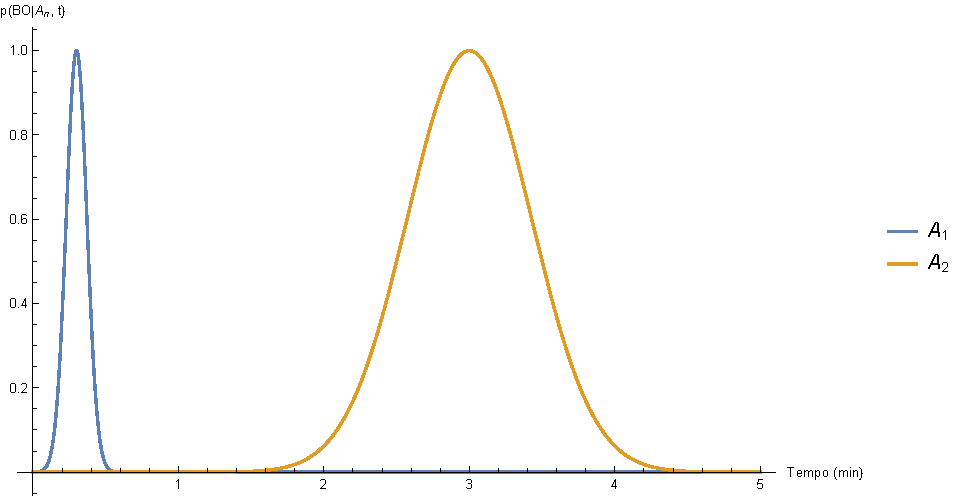
\includegraphics[width=\linewidth]{../Mathematica/Distribuicao1.pdf}
	\end{center}
\end{figure}

Na Figura \ref{fig:rev-distribuicao-exemplo} é possível observar que a primeira vez que a ação é executada, a tolerância para atraso é pequena, contudo, na segunda execução a tolerância de atraso é muito maior, pois o efeito da \gls{tech-tree} implica que uma ação atrasada irá atrasar as duas ações dependentes.

A tolerância de execução se faz necessária pois um jogador pode atrasar alguns segundos por múltiplos motivos durante o jogo, embora ele ainda esteja executando a mesma build-order.

Para uma \textit{\gls{build-order}} real, haverá uma distribuição de probabilidade para cada uma das ações que podem oscilar em torno de 30 a 40 dependendo da facção do jogador.

%-------------------------------------------------------------------------
		\section{Fator de \textit{branching} de um jogo de StarCraft: BroodWar}
%-------------------------------------------------------------------------
Em teoria dos jogos \todo{referencia}, \textit{branching factor} é o número de nós-filho em cada um dos nós de ações possíveis no jogo, isto é, é o número de opções que um jogador tem disponível em cada momento.

Infelizmente não há análises cientificas feitas para a complexidade de um jogo de StarCraft II, mas é possível realizar uma comparação utilizando o jogo antecessor da série, StarCraft: Brood War lançado em 1998. De acordo com \cite{weber2009data}, StarCraft: BroodWar possui um fator de branching estimado médio de $1 \times 10^6$ que, comparado à um jogo de xadrez onde a média é de 35, é um valor extremamente alto. O alto nível de complexidade força que seja utilizado um modelo probabilístico ao invés de uma análise determinista, uma vez que é impossível obter, ou sequer gerar, uma amostra para todas as possibilidades de jogos. Devido a novas mecânicas de jogo introduzidas em StarCraft II espera-se a complexidade seja superior à de seu antecessor.

%-------------------------------------------------------------------------
		\section{O Teorema de Bayes}
%-------------------------------------------------------------------------
O Teorema de Bayes relaciona a probabilidade de um evento associado à uma restrição. A definição matemática do teorema é dada pela Equação \ref{eq:revisao-teorema-bayes}:

\begin{equation}
	P(A|B) = \frac{P(B|A)P(A)}{P(B)}
	\label{eq:revisao-teorema-bayes}
\end{equation}

\noindent onde $A$ é um evento, $B$ é a restrição do evento $A$. Dessa forma, é possível determinar a probabilidade do evento $A$ ter acontecido, dado que o evento $B$ foi observado.

Em termos da análise de \textit{\glspl{build-order}}, pode-se aplicar o teorema conforme a Equação \ref{eq:revisao-teorema-bayes-aplicado}:

\begin{equation}
	P(BO|A, t) = \frac{P(A|BO, t)P(BO)}{P(A, t)}
	\label{eq:revisao-teorema-bayes-aplicado}
\end{equation}
\noindent onde $BO$ é uma \textit{\gls{build-order}} qualquer que deseja-se estimar a probabilidade de estar sendo executada, dado que o jogador executou a ação $A$ no tempo $t$. Para tanto, precisa-se determinar 3 fatores:

\begin{itemize}
	\item $P(A, t)$: a probabilidade de um jogador executar a ação $A$ no instante $t$, independe da \textit{\gls{build-order}};
	\item $P(BO)$: a probabilidade de um jogador executar a \textit{\gls{build-order}} $BO$, independente da ação que o jogador está executando;
	\item $P(A|BO, t)$: a probabilidade de ter executado a ação $A$ supondo que o jogador está executando a \textit{\gls{build-order}} $BO$ no instante $t$;
\end{itemize}

%=========================================================================
% METODOLOGIA EXPERIMENTAL
	\chapter{Método}
%=========================================================================
Neste trabalho foi utilizado Python 2.7 como a linguagem de programação para a implementação do método. Este motivo foi guiado principalmente pelo fato da biblioteca oficial de processamento de \glspl{replay} oferecida pela Blizzard Entertainment, Inc. (desenvolvedor do StarCraft II) ser em Python. A biblioteca de processamento de \glspl{replay} oficial, \textit{s2protocol}\cite{s2protocol} é de código-fonte aberto e está disponível no GitHub. Demais códigos utilizados são parte de uma distribuição padrão do Python 2.7 ou foram desenvolvidos para o trabalho.

%-------------------------------------------------------------------------
		\section{Extração dos dados}
%-------------------------------------------------------------------------

Os \glspl{replay} de StarCraft II são arquivos do tipo MoPAQ, um formato proprietário desenvolvido pela Blizzard Entertainment nos anos 90 para uso em seus jogos. Embora o formato seja proprietário é possível localizar na internet uma gama de implementações ou documentação desenvolvida por engenharia reversa. Um arquivo MPQ é análogo à um arquivo ZIP e contém um índice de arquivos e blocos de conteúdo. Nos \textit{\glspl{replay}} há uma série de \textit{stream} de eventos de jogo e neste trabalho somente será utilizado o stream chamado "Tracker Events" que são eventos cujo conteúdo é destinado para ferramentas que desejam processar os \glspl{replay}, ao contrário de informações úteis para a simulação do jogo. Este \textit{stream} está armazenado como "replay.tracker.events" dentro do MPQ.

O \textit{stream} de \textit{Tracker Events} foi processado utilizando uma classe em Python que extrai as seguintes informações do evento:

\begin{itemize}
	\item Nome (tipo) do evento;
	\item \textit{Game loop} do evento (o número de iterações do loop principal do jogo);
	\item ID do jogador que gerou o evento;
	\item Estrutura de dados específica de cada evento;
\end{itemize}

A expressão de conversão de \textit{game loops} para o tempo, em segundos é dada pela Equação \ref{eq:metodo-conversao-loops-tempo}.

\begin{equation}
	t_{seg} = 16 \cdot n_{loops} \cdot \frac{26}{36} \cdot \frac{131}{148}
	\label{eq:metodo-conversao-loops-tempo}
\end{equation}
\noindent onde $t_{seg}$ é o tempo em segundos, $n_{loops}$ é o número de \textit{game loops}.

Dentre os vários tipos de eventos contidos neste stream, 3 destes eventos são interessantes na análise:

\begin{description}
	\item[NNet.Replay.Tracker.SUnitBornEvent] evento disparado para cada \gls{unidade}/\gls{estrutura} criada no jogo. Este evento somente é despachado para \glspl{unidade} que aparecem no campo de batalha de forma "pronta", isto é, no momento em que a \gls{unidade} pode ser vista pelo jogador, ela já pode ser controlada.
	\item[NNet.Replay.Tracker.SUnitInitEvent] semelhante ao evento SUnitBornEvent, mas este evento é despachado para \glspl{unidade} que são construídas diretamente no campo de batalha e não estão disponíveis para jogo imediatamente no instante do evento. Embora a \gls{unidade}/\gls{estrutura} neste evento não seja imediatamente utilizável, no método proposto, apenas o tempo em que usuário inicia a construção é considerado.
	\item[NNet.Replay.Tracker.SUpgradeEvent] evento disparado para cada \gls{melhoramento} de exército realizado pelo jogador. Estes eventos são muito importantes pois podem indicar ou refinar a intenção do jogador.
\end{description}

Apenas uma informação é extraída da \gls{estrutura} de dados específica dos eventos: o nome da \gls{unidade}, \gls{estrutura} ou \gls{melhoramento} feito pelo jogador. Este nome é único para cada tipo de \gls{unidade}, \gls{estrutura} ou \gls{melhoramento} e cada um desses nomes são considerados como ações individuais que podem ser executadas pelo jogador. A única exceção é a exclusão de \glspl{unidade} do tipo trabalhadoras e \glspl{estrutura} que oferecem suprimento ao jogador. Estas \glspl{unidade} foram removidas porque num jogo regular estas ações ocorrem muitas vezes e há muita variância na execução delas, logo, incorrendo num prejuízo na qualidade do resultado final.

Uma vez que após os 6 minutos de jogo, a partida se torna reativa, ao invés de algorítmica, a sequência de eventos é truncada até os 6 minutos de jogo. Isto garante que as informações tenham menor variabilidade. Ao decorrer da partida, as ações executadas por um jogador começam a se tornar em resposta das ações do outro jogador e, portanto, não há sentido realizar uma classificação de \textit{\gls{build-order}} para ações que ocorrem além de um certo limite de tempo.

%-------------------------------------------------------------------------
		\section{\textit{Dataset} de referência}
%-------------------------------------------------------------------------
Como não há nenhum índice de \glspl{replay} e \glspl{build-order} disponível publicamente o conjunto de \glspl{replay} utilizado para treinamento e validação foi classificado manualmente utilizando \glspl{replay} de diversos campeonatos do ano de 2016

\begin{description}
	\item[Intel Extreme Masters 10]: 19 \textit{\glspl{replay}}
	\item[Intel Extreme Masters 11]: 35 \textit{\glspl{replay}}
	\item[WCS Spring Championship 2016]: 54 \textit{\glspl{replay}}
\end{description}

\noindent totalizando $108$ \textit{\glspl{replay}}.

Para a classificação manual das estratégias cada \gls{replay} foi assistido no jogo e classificado conforme as regras abaixo:

\begin{itemize}
	\item A composição de exército de um jogador no instante do primeiro ataque realizado por ele;
	\item Se o jogador fosse atacado por outro e tivesse mais de 8 \glspl{unidade} perdidas, o \textit{\gls{replay}} era descartado;
	\item Caso não houvesse investida por parte dos dois jogadores até os 6 minutos de jogo, a composição de exército do jogador aos 6 minutos de jogo era classificada.
\end{itemize}

Um exército em StarCraft II pode ser composto por mais de 10 tipos de \glspl{unidade} diferentes, contudo isto é incomum. De forma geral, exércitos são compostos por um grande número de \glspl{unidade} básicas de ataque e algumas \glspl{unidade} de suporte. Na classificação, as \glspl{unidade} de suporte foram desprezadas na composição do exército. Esta regra é violada somente caso a \gls{unidade} de suporte seja incomum ou trouxe um benefício significante para o jogador, como estratégias do tipo \textit{rush} (criar um exército o mais rápido possível, geralmente em sacrifício da economia).

%-------------------------------------------------------------------------
		\section{Treinamento}
		\label{sec:treinamento}
%-------------------------------------------------------------------------

O treinamento foi realizado de forma simples: a sequência de ações para cada \textit{\gls{replay}} era iterada e o tempo de execução da ação era gravado em uma lista. Uma lista separada era usada para cada \gls{repeticao}. Por exemplo, supondo que as \textit{\glspl{build-order}} $BO_1$ e $BO_2$ sejam duas amostras com o mesmo \textit{label}:

\begin{table}[H]
\centering
\caption{Um exemplo de uma \textit{\gls{build-order}} com as ações $A_1$ e $A_2$ ocorrendo nos tempos $t_n$. Observa-se nas últimas 2 linhas da tabela que há uma inversão de sequência de execução das ações. Esta alteração não implica que as \textit{\gls{build-order}} sejam diferentes, é muito provável que os tempos $t_5$, $t_6$, $t_7$ e $t_8$ sejam muitos próximos e são independentes.}
\label{my-label}
\begin{tabular}{|l|l||l|l|}
\hline
\multicolumn{2}{|l||}{\centering $BO_1$} & \multicolumn{2}{l|}{\centering $BO_2$} \\ \hline
\textbf{T}  & \textbf{A}  & \textbf{T}  & \textbf{A} \\ \hline
$t_1$       & $A_1$       & $t_2$       & $A_1$      \\ \hline
$t_3$       & $A_1$       & $t_4$       & $A_1$      \\ \hline
$t_5$       & $A_2$       & $t_6$       & $A_1$      \\ \hline
$t_7$       & $A_1$       & $t_8$       & $A_2$      \\ \hline
\end{tabular}
\end{table}

Dessa forma, as duas listas terão o seguinte conteúdo:

\begin{align}
\begin{split}
    T_{A_1} = \{
		&\{t_1, t_2\}, 		\\
		&\{t_3, t_4\}, 		\\
		&\{t_6, t_7\}
	\}
\end{split}
\label{eq:metodo-exemplo-vetor-tempos-a1}
\end{align}
\noindent onde $T_{A_1}$ é o vetor de tempos da execução de cada \gls{repeticao} da ação $A_1$ nos múltiplos \textit{\glspl{replay}} processados. $\{t_1, t_2\}$ representa os tempos da primeira \gls{repeticao}, $\{t_3, t_4\}$ da segunda e $\{t_6, t_7\}$ da terceira.

\begin{align}
\begin{split}
    T_{A_2} = \{
		&\{t_5, t_8\}
	\}
\end{split}
\label{eq:metodo-exemplo-vetor-tempos-a2}
\end{align}
\noindent onde $T_{A_2}$ é o vetor de tempos da execução de cada \gls{repeticao} da ação $A_2$ nos múltiplos \textit{\glspl{replay}} processados. Esta ação possui uma única \gls{repeticao}.

Seja $\mu(T_x, R)$ a média do vetor de tempo $T_x$ para a \gls{repeticao} $R$ e $\sigma(T_x, R)$ o desvio padrão do vetor de tempo $T_x$ para a \gls{repeticao} $R$, então a distribuição $p$ de probabilidade de uma ação pode ser definida como:

\begin{equation}
	p_{T_x}(t, R) = A e^{-\frac{(t-\mu(T_x, R))^2}{{\sigma(T_x, R)}^2}}
	\label{eq:metodo-funcao-distribuicao-de-probabilidade}
\end{equation}
\noindent onde $A$ é a frequência com que um par ação-\gls{repeticao} ocorre dentre todas as amostras de treinamento utilizadas, $\mu$ é o tempo médio de execução do par ação-\gls{repeticao} e $\sigma$ e o correspondente desvio-padrão.

A Equação \ref{eq:metodo-funcao-distribuicao-de-probabilidade} apresenta a função distribuição de probabilidade para uma ação. Isto é, representa a probabilidade de uma ação qualquer $A$ pertencer a uma \textit{\gls{build-order}} $BO_1$ dado que a ação foi executada pelo jogador no instante $t$.

Esta função é uma variação da função distribuição de probabilidade Gaussiana, no entanto, é ajustada de forma que, para o ponto médio, seu valor seja unitário (para $A=1$) ou tenha o valor de $A$, que indica a frequência com que uma ação ocorreu nos \textit{datasets} de treinamento.

Para o cálculo da média ($\mu$) e desvio padrão ($\sigma$) os itens internos do vetor $T_x$ são utilizados. Para o exemplo apresentado nas Equações \ref{eq:metodo-exemplo-vetor-tempos-a1} e \ref{eq:metodo-exemplo-vetor-tempos-a2}, as médias são dadas pelos vetores das Equações \ref{eq:metodo-exemplo-vetor-tempos-a1-media} e \ref{eq:metodo-exemplo-vetor-tempos-a2-media}, respectivamente:

\begin{equation}
    \mu_{A_1} = \left\{
		\frac{t_1 + t_2}{2}, 
		\frac{t_3 + t_4}{2}, 		
		\frac{t_6 + t_7}{2}
	\right\}
	\label{eq:metodo-exemplo-vetor-tempos-a1-media}
\end{equation}

\begin{equation}
    \mu_{A_1} = \left\{
		\frac{t_5 + t_8}{2}
	\right\}
	\label{eq:metodo-exemplo-vetor-tempos-a2-media}
\end{equation}

O cálculo de desvio padrão para os vetores das Equações \ref{eq:metodo-exemplo-vetor-tempos-a1} e \ref{eq:metodo-exemplo-vetor-tempos-a2} foi omitido no exemplo pois a expressão é complexa e não influencia no entendimento e um valor genérico é apresentado nas Equações \ref{eq:metodo-exemplo-vetor-tempos-a1-desvio} e \ref{eq:metodo-exemplo-vetor-tempos-a2-desvio}.

\begin{equation}
    \sigma_{A_1} = \left\{
		\sigma_{{A_1},1}, 
		\sigma_{{A_1},2}, 	
		\sigma_{{A_1},3}
	\right\}
	\label{eq:metodo-exemplo-vetor-tempos-a1-desvio}
\end{equation}

\begin{equation}
    \sigma_{A_1} = \left\{
		\sigma_{{A_2},1}
	\right\}
	\label{eq:metodo-exemplo-vetor-tempos-a2-desvio}
\end{equation}

Neste exemplo, de forma a simplificar o cálculo, assume-se que a frequência de cada par ação-\gls{repeticao} é unitária.

É possível substituir os valores de média e desvio-padrão das Equações \ref{eq:metodo-exemplo-vetor-tempos-a1-media}, \ref{eq:metodo-exemplo-vetor-tempos-a2-media}, \ref{eq:metodo-exemplo-vetor-tempos-a1-desvio} e \ref{eq:metodo-exemplo-vetor-tempos-a2-desvio} na função distribuição de probabilidade da Equação \ref{eq:metodo-funcao-distribuicao-de-probabilidade}. O vetor final é denominado de "vetor de probabilidades".

Com os resultados de média (Equações \ref{eq:metodo-exemplo-vetor-tempos-a1-media} e \ref{eq:metodo-exemplo-vetor-tempos-a2-media}) e desvio padrão (Equações \ref{eq:metodo-exemplo-vetor-tempos-a1-desvio} e \ref{eq:metodo-exemplo-vetor-tempos-a2-desvio}), é possível obter um gráfico do formato da distribuição de probabilidade conforme representado nas Figuras \ref{fig:metodo-exemplo-bo-media-a1} e \ref{fig:metodo-exemplo-bo-media-a2}.

\begin{figure}[htb]
	\caption{\label{fig:metodo-exemplo-bo-media-a1} Exemplo da distribuição de probabilidade da ação $A_1$. A curva em azul representa a primeira \gls{repeticao} da ação (nos tempos $t_1$ e $t_2$), a curva em laranja representa a segunda \gls{repeticao} (nos tempos $t_3$ e $t_4$) e a curva em verde representa a terceira \gls{repeticao} da ação (tempos $t_6$ e $t_7$).}
	\begin{center}
	    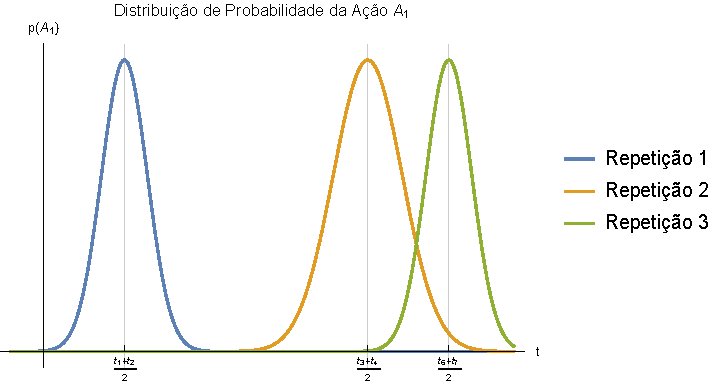
\includegraphics[width=\linewidth]{../Mathematica/Images/Exemplo_BO_Media_A1.pdf}
	\end{center}
\end{figure}

\begin{figure}[htb]
	\caption{\label{fig:metodo-exemplo-bo-media-a2} Exemplo da distribuição de probabilidade da ação $A_1$. Como a ação $A_2$ somente é executada uma única vez no exemplo, apenas uma \gls{repeticao} é mostrada no gráfico. A ação corresponde aos instantes de tempo $t_5$ e $t_8$.}
	\begin{center}
	    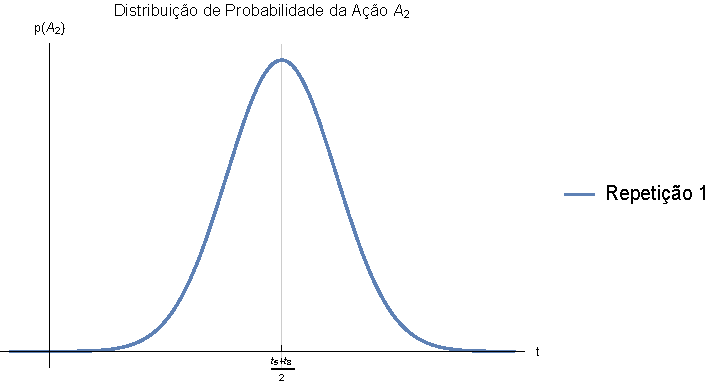
\includegraphics[width=\linewidth]{../Mathematica/Images/Exemplo_BO_Media_A2.pdf}
	\end{center}
\end{figure}

%-------------------------------------------------------------------------
			\subsection{Forma Matricial}
%-------------------------------------------------------------------------
O treinamento pode ser realizado de forma matricial. Onde as colunas indicam as ações e as linhas indicam as \glspl{repeticao} de cada ação respectiva. Dessa forma, é possível definir uma matriz de médias e desvios padrões.

Dado um conjunto de $N$ ações que podem se repetir até $M$ vezes, então, é possível definir uma matriz $M \times N$, cujos elementos são formatos pelo tempo médio de execução de cada par ação-\gls{repeticao}, denominada de "matriz de média do tempo de execução", expressa na Equação \ref{eq:metodo-matriz-media-simbolico}.

\newcommand{\RogielBOMatrix}[1]{
	\ensuremath{
		\left(\begin{array}{cccc}
 			{#1}_{A_1,1} & {#1}_{A_2,1} & \cdots & {#1}_{A_N,1} \\
 			{#1}_{A_1,2} & {#1}_{A_2,2} & \cdots & {#1}_{A_N,2} \\
 			\vdots 		 & \vdots 	    & \ddots & \vdots 		\\
 			{#1}_{A_1,M} & {#1}_{A_2,M} & \cdots & {#1}_{A_N,M}
		\end{array}\right)
	}
}

\begin{equation}
	\mu = \RogielBOMatrix{\mu}
	\label{eq:metodo-matriz-media-simbolico}
\end{equation}

De forma análoga a matriz de média do tempo de execução, é possível definir a "matriz de desvio padrão do tempo de execução" para os valores de desvio padrão do tempo de execução de cada par ação-\gls{repeticao} e a outra matriz denominada "matriz de frequência de ocorrência de \gls{repeticao}" que define a frequência de ocorrência de um dado par ação-\gls{repeticao} no conjunto de amostras observadas. A definição formal da matriz de desvio padrão do tempo de execução está apresentada na Equação \ref{eq:metodo-matriz-desvio-simbolico}. A definição formal da matriz de frequência de \gls{repeticao} está apresentada na Equação \ref{eq:metodo-matriz-frequencia-simbolico}.

\begin{equation}
	\sigma = \RogielBOMatrix{\sigma}
	\label{eq:metodo-matriz-desvio-simbolico}
\end{equation}

\begin{equation}
	F = \RogielBOMatrix{F}
	\label{eq:metodo-matriz-frequencia-simbolico}
\end{equation}


Substituindo-se as matrizes de média e desvio padrão do tempo de execução e de frequência de ocorrência de \gls{repeticao}, Equações \ref{eq:metodo-matriz-media-simbolico}, \ref{eq:metodo-matriz-desvio-simbolico} e \ref{eq:metodo-matriz-frequencia-simbolico}, respectivamente, na função de distribuição de probabilidade dada pela Equação \ref{eq:metodo-funcao-distribuicao-de-probabilidade}, é possível construir uma matriz de probabilidade. Todas as operações entre matrizes são realizadas utilizando operadores de Hadamard \cite{matrix-analysis} ou operações termo-a-termo.

Por convenção matemática, e para evitar um problema de indeterminação no cálculo de probabilidade associada, uma ação cuja \gls{repeticao} não ocorre nas amostras encontradas, deve ter o valor de média não-nulo e o valor de desvio padrão deve ser infinito. Por convenção, neste trabalho utiliza-se o valor de média $0.0$. Esta escolha foi feita para que a função distribuição de probabilidade seja avaliada com valor $1.0$ para ações inexistentes na amostra de treinamento, independente da ação ser executada pelo jogador numa \textit{\gls{build-order}} utilizada no processo de classificação.

\newcommand{\RPME}[4]{
	\ensuremath{
		{#1} e^{-\frac{(#4-{#2})^2}{{{#3}}^2}}
	}
}
\newcommand{\RPMGE}[1]{
	\RPME{F_{{#1}}}{\mu_{{#1}}}{\sigma_{{#1}}}{t_{{#1}}}
}


\begin{equation}
	p(t) = \left(
		\begin{array}{cccc}
			\RPMGE{A_1,1} & \RPMGE{A_2,1} & \cdots & \RPMGE{A_N,1} \\
 			\RPMGE{A_1,2} & \RPMGE{A_2,2} & \cdots & \RPMGE{A_N,2} \\
 			\vdots 	  	  & \vdots 	  	  & \ddots & \vdots 	       \\
 			\RPMGE{A_1,M} & \RPMGE{A_2,M} & \cdots & \RPMGE{A_N,M}
		\end{array}
	\right)
	\label{eq:metodo-matriz-probabilidade-simbolico}
\end{equation}
\noindent onde $t$ é uma matriz que indica o tempo de execução dos pares ação-\gls{repeticao} de uma \textit{\gls{build-order}} que se deseja classificar.

%-------------------------------------------------------------------------
		\section{Classificação}
		\label{sec:classificacao}
%-------------------------------------------------------------------------
O processo de classificação é realizado de forma independente para cada \textit{label} (\textit{\gls{build-order}}) utilizado no processo de treinamento. Os valores de probabilidade para cada par de ação-tempo de um \textit{\gls{replay}} são multiplicados e o valor final determina a semelhança de uma \textit{\gls{build-order}} treinada e a executada.

Considerando-se o exemplo anterior, é possível aplicar o instante de execução de cada ação do jogador no vetor de ações correspondente e obter a probabilidade de que uma ação qualquer $A$. Dessa forma, a probabilidade total de que um conjunto de ações seja parte de uma \textit{\gls{build-order}} qualquer é dada pela Equação \ref{eq:metodo-exemplo-classificacao-produto}:

\begin{equation}
	p_{BO} = \prod_{n,i} p(BO|A_{(n,i)}, t)
	\label{eq:metodo-exemplo-classificacao-produto}
\end{equation}
\noindent onde $n$ indica o tipo da ação, $i$ a sua \gls{repeticao} e $p(BO|A_{(n,i)}, t)$ é a probabilidade de que a ação seja parte de uma \gls{build-order} $BO$ dado que $A_{(n,i)}$ foi executada no instante de tempo $t$, conforme a Equação \ref{eq:metodo-funcao-distribuicao-de-probabilidade}.

%-------------------------------------------------------------------------
			\subsection{Forma Matricial}
%-------------------------------------------------------------------------
Dada a matriz de probabilidades de uma \textit{\gls{build-order}} treinada, conforme a Equação \ref{eq:metodo-matriz-probabilidade-simbolico}, a probabilidade final de uma \textit{\gls{build-order}} treinada é dada pela redução da matriz através da operação de multiplicação de seus termos, conforme Equação \ref{eq:metodo-matriz-reducao}.

\begin{equation}
	p_{BO} = \prod_{i,j} p(t)_{ij}
	\label{eq:metodo-matriz-reducao}
\end{equation}
\noindent onde $i$ e $j$ são respectivamente as linhas e as colunas das matrizes de probabilidade e de tempo de execução da \textit{\gls{build-order}} a ser classificada, $t$ é a matriz de tempo de execução da \textit{\gls{build-order}} para ser classificada, $p$ é a matriz de probabilidades de uma \textit{\gls{build-order}} qualquer $BO$ e $p_{BO}$ é a probabilidade reduzida da matriz $p$ cujo valor é equivalente à operação da Equação \ref{eq:metodo-exemplo-classificacao-produto}.

%-------------------------------------------------------------------------
		\section{Implementação}
%-------------------------------------------------------------------------

A implementação do método foi feita em Python 2.7 utilizando a biblioteca s2protocol \cite{s2protocol} para processamento dos arquivos de \textit{\gls{replay}}, disponibilizada em licença de código fonte aberto no GitHub.

Para realizar a extração dos eventos do uma função chamada \textit{\textit{parse()}} foi definida. Esta função é responsável por extrair todas a \textit{\glspl{build-order}} de todos jogadores que participaram na partida contida num arquivo de \textit{\gls{replay}}. A função pode ser dividida em 3 etapas.

Na primeira etapa, extrai-se do cabeçalho do arquivo informações que associam um identificador inteiro, denominado de \textit{player ID} com o nome do jogador e a \gls{raca}. O identificador inteiro é usado nas estruturas de dados dos eventos para associar o evento com um jogador. Com estes dados, é construído um dicionário contendo as seguintes informações.

\begin{lstlisting}
players = {
	playerID: {
		'Name':       ..., // nome do jogador
		'BuildOrder': ..., // estrutura que lista as ações da build order
		'Race':       ...  // nome da raça do jogador
	}
}
\end{lstlisting}

Depois de criada a estrutura de dados do jogador, é possível realizar a extração de cada evento do \textit{\gls{replay}}. Para cada estrutura de dados de evento recebida pela biblioteca de processamento conforme o exemplo abaixo:

\begin{lstlisting}
	{'_bits': 296,
	 '_event': 'NNet.Replay.Tracker.SUnitBornEvent',
	 '_eventid': 1,
	 '_gameloop': 2467,
	 'm_controlPlayerId': 2,
	 'm_unitTagIndex': 261,
	 'm_unitTagRecycle': 1,
	 'm_unitTypeName': 'Adept',
	 'm_upkeepPlayerId': 2,
	 'm_x': 34,
	 'm_y': 152}
\end{lstlisting}

Antes de processar qualquer elemento do evento, converte-se o campo \_gameloop que representa o número de loops de jogo transcorridos até o momento do evento. A conversão para tempo em segundos é feita utilizando a expressão da Equação \ref{eq:metodo-conversao-loops-tempo}. Se o tempo de execução é superior à 6 minutos, o evento é descartado.

Caso o tempo seja inferior ou igual à 6 minutos, checa-se o tipo de evento. Se o evento for do tipo \textbf{SUnitBornEvent}, \textbf{SUnitInitEvent} ou \textbf{SUpgradeEvent} extrai-se alguns atributos da sua estrutura de evento. Caso contrário, o evento é descartado.

Se o evento for do tipo \textbf{SUnitBornEvent} ou \textbf{SUnitInitEvent}, então extrai-se do campo m\_unitTypeName o nome da \gls{unidade} treinada e a ID do jogador que executou a ação, contida em m\_upkeepPlayerId. A ID é usada para obter a estrutura de \gls{build-order} apresentada anteriormente e uma ação com nome m\_unitTypeName e tempo de execução correspondente à \_gameloop é adicionada na estrutura de dados de \gls{build-order} do jogador.

Se o evento for do tipo \textbf{SUpgradeEvent}, então extrai-se do campo m\_upgradeTypeName o nome do \gls{melhoramento} executado e a ID do jogador que executou a ação, contida em m\_playerId. A ID é usada para obter a estrutura de \gls{build-order} apresentada anteriormente e uma ação com nome m\_upgradeTypeName e tempo de execução correspondente à \_gameloop é adicionada na estrutura de dados de \gls{build-order} do jogador.

Nem todos valores de m\_unitTypeName ou m\_upgradeTypeName são válidos e é necessário checar em uma lista de valores permitidos antes que os valores sejam adicionados à estrutura de dados de \gls{build-order} do jogador. A lista de todas ações permitidas estão no Anexo \ref{an:lista-acoes}.

É importante observar que não há sobreposição entre os nomes de \glspl{unidade} treinadas em m\_unitTypeName e os nomes dos \glspl{melhoramento} feitos em m\_upgradeTypeName e portanto os próprios nomes são utilizados como ações. Isto é, conforme o exemplo dado, a sua ação correspondente no processo de treinamento do método é chamada de \gls{adept} pois é o valor contido no campo m\_unitTypeName.

Após a construção da estrutura de dados de uma \textit{\gls{build-order}}, é possível executar o algoritmo de treinamento. Este algoritmo é responsável pelo cálculo de média e desvio padrão de cada ação coletada na etapa anterior. O cálculo é feito conforme descrito na seção \ref{sec:treinamento}.

O classificador foi implementado numa classe em Python chamada de \textit{BuildOrderMatcher}. Esta classe é responsável pela organização das estruturas de dados do treinamento e classificação das \textit{\glspl{build-order}}.

O processo de treinamento foi implementado num método denominado \textit{train()} na classe \textit{BuildOrderMatcher} onde é dado um conjunto de estruturas de \textit{\gls{build-order}}, conforme extraído pelo método descrito na função \textit{parse()}, e um \textit{label} que identifica o nome que representa o conjunto de \textit{\glspl{build-order}} dado. A função de treino itera sobre cada uma das \textit{\glspl{build-order}} dadas e acumula o tempo de execução de cada uma das ações em termos das suas \glspl{repeticao} em uma lista. A \gls{repeticao} é definida como a sequência em que uma mesma ação é executada. Se uma ação é executada ao total 3 vezes numa \textit{\gls{build-order}}, então a primeira vez que ela é executada é definida como a repetição 1, a segunda vez que ela é executada é definida como a repetição 2 e a terceira como a repetição 3. Os valores de tempo de cada par ação-repetição são adicionados em uma estrutura de dicionário com 3 níveis. O primeiro nível representa o \textit{label} de treinamento, o segundo nível representa o nome a ação e o terceiro nível representa a repetição.

Após a adição de todas \textit{\glspl{build-order}} e seus \textit{labels} pelo método \textit{train()} da classe \textit{BuildOrderMatcher}, um segundo método \textit{build\_distribution()} deve ser invocado para que sejam geradas as funções distribuição de probabilidade conforme a Equação \ref{eq:metodo-funcao-distribuicao-de-probabilidade}. Esta função é responsável pelo cálculo dos parâmetros da função distribuição de probabilidade. Um conjunto distinta de atributos da função distribuição de probabilidade é calculado e associado a cada par ação-repetição para cada \textit{label} dado no método \textit{train()}.

A função \textit{build\_distribution()} itera por repetição de cada ação de cada um dos labels dados em \textit{train()} e verifica que o par ação-repetição ocorre em pelo menos 2 amostras, caso contrário não seria possível atribuir um valor de desvio padrão para o par. Se há ao menos 2 elementos, calcula-se o parâmetro $A$ da Equação \ref{eq:metodo-funcao-distribuicao-de-probabilidade} pelo tamanho de elementos (valores de tempo em segundos em que cada amostra executou uma ação, se uma ação não foi executada em alguma amostra, a lista possui um item a menos). O parâmetro é calculado dividindo-se o número de elementos de tempo na lista do par ação-repetição pelo número total de \textit{\glspl{build-order}} dada para treinamento. De forma que, se um par ação-repetição ocorre em todas as amostras, seu valor é de $1.0$ ou se um par ação-repetição ocorre em apenas duas de dez amostras de treinamento, seu valor é de $0.2$.

Por fim, calcula-se o valor de média e desvio padrão do tempo de execução de cada par e constrói-se um objeto que representa de forma abstraída a função distribuição de probabilidade utilizando os parâmetros $A$, $\mu$ e $\sigma$. Ao invocar o método \textit{apply()} com um valor de tempo $t$, é retornado o valor correspondente da função distribuição de probabilidade.

\begin{lstlisting}[breaklines=true]
	class NormalDistributionFunction:
    	def __init__(self, mean, sigma=1.0, amplitude=1.0):
        	self.mean = mean
        	self.sigma = sigma
        	self.amplitude = amplitude

    	def apply(self, t):
        	if t is None:
            	return 0.0
        	return self.amplitude * math.exp(-(math.pow(t-self.mean, 2) / (2 * math.pow(self.sigma, 2))))
\end{lstlisting}

O objeto representando a função distribuição de probabilidade é adicionado à uma estrutura de dicionário com 3 níveis. O primeiro nível representa o \textit{label} de treinamento, o segundo nível representa o nome a ação e o terceiro nível representa a repetição.

Após a chamada do método \textit{build\_distribution()} a classe está pronta para classificação de outras \textit{\glspl{build-order}} desconhecidas através do método \textit{classify()} onde é dado a estrutura de dados de uma \textit{\gls{build-order}} desconhecida e o algoritmo calcula os valores de probabilidade associada à cada \textit{label}. O cálculo é feito conforme descrito na seção \ref{sec:classificacao}.

O método \textit{classify()} itera nos \textit{labels} de treinamento e itera sobre a sequência de ações executadas na \textit{\gls{build-order}} dada. Um contador é mantido por \textit{label} e por ação que indexa o índice de repetição que é incrementado a cada ocorrência de uma ação com mesmo nome. Com isto, dado o \textit{label} da iteração, a ação ta iteração e o índice da repetição da ação, pode-se utilizar a função distribuição de probabilidade e calcular o valor de probabilidade associado ao par ação-repetição. O valor invidual de probabilidade de cada par é multiplicado pelo valor total de probabilidade do \textit{label}. A função retorna um dicionário indexado pelo \textit{label} e cujo valor é produto das probabilidades.

A seleção da \textit{\gls{build-order}} correta é feita escolhendo o label que possui o maior valor de probabilidade agregada.

%=========================================================================
% RESULTADOS E DISCUSSÕES
	\chapter{Resultados e Discussões}
%=========================================================================

No processo de treinamento, é extraído a sequência de construção de cada jogador (a \textit{\gls{build-order}}), calculadas estatísticas de primeira ordem (média e desvio padrão) e a frequência de cada par ação-\gls{repeticao} em relação ao conjunto de \glspl{replay} correspondentes a mesma \textit{\gls{build-order}}.

No processo de classificação, as probabilidades individuais de cada ação executada são calculadas e multiplicadas para obter um número que indica a probabilidade de que uma dado conjunto de ações pertença à uma \textit{\gls{build-order}} conhecida.

O método foi treinado utilizando 7 \gls{build-order} da \gls{raca} \Gls{protoss}.

\begin{description}
	\item[Adept Glaives]: 6 \glspl{replay}
	\item[Adept Stargate]: 14 \glspl{replay}
	\item[Adept Immortal]: 13 \glspl{replay}
	\item[Stalker Immortal]: 3 \glspl{replay}
	\item[Adept Prism DT]: 5 \glspl{replay}
	\item[Stalker Disruptor]: 5 \glspl{replay}
	\item[Blink Stalker]: 8 \glspl{replay}
\end{description}

A Figura \ref{fig:resultados-protoss-immortal-gateway} apresenta um exemplo das funções distribuição de probabilidade para uma ação do tipo "Gateway" da \textit{\gls{build-order}} "Adept Immortal".

\begin{figure}[htb]
	\caption{\label{fig:resultados-protoss-immortal-gateway} Forma gráfica de distribuição estatística de uma ação \textit{Gateway} e suas \glspl{repeticao}}
	\begin{center}
	    \includegraphics[width=\linewidth]{{"../Classifier/Graphs/Protoss/Adept Immortal"}/Gateway.png}
	\end{center}
\end{figure}

Observa-se que a frequência de ocorrência das \glspl{repeticao} no \textit{dataset} de treinamento é decrescente. Isto é uma consequência do método escolhido para classificação. A primeira execução de uma ação, irá, independentemente do tempo em que for executada, considerada como a primeira \gls{repeticao}. A redução da frequência tem duas causas principais:

\begin{description}
	\item[Alteração da estratégia do jogador]: um jogador pode ter escolhido uma estratégia levemente diferente devido ao contexto do jogo ou em resposta à \textit{\gls{build-order}} do oponente;
	\item[Ações opcionais]: algumas ações podem ser opcionais e somente são executadas em alguns mapas. 
\end{description}

Há uma tendência no desvio-padrão e variância do tempo de execução do par ação-\gls{repeticao} de crescerem ao decorrer da partida. Os principais motivos deste crescimento é a incapacidade de jogadores humanos executarem as ações de forma perfeita e sem qualquer variabilidade. Este fator é agravado com a característica da "\gls{tech-tree}" onde algumas ações possuem dependências tecnológicas em outras anteriores. Embora a tendência seja visível na maior parte das ações, ainda é possível que ela reduza em alguns casos específicos.

Um exemplo onde o desvio padrão reduz de forma significante é visível na Figura \ref{fig:resultados-protoss-immortal-adept}, a primeira \gls{repeticao} possui um desvio padrão significantemente maior ao da segunda \gls{repeticao}. Este comportamento é esperado quando a primeira ação é considerada opcional e incorre num erro onde a primeira \gls{repeticao} deveria ter frequência menor que a segunda. Infelizmente, devido à forma de como o método de separação foi estabelecido, não é possível evitar este efeito.

\begin{figure}[htb]
	\caption{\label{fig:resultados-protoss-immortal-adept} Forma gráfica de distribuição estatística de uma ação \textit{Adept} e suas \glspl{repeticao}}
	\begin{center}
	    \includegraphics[width=\linewidth]{{"../Classifier/Graphs/Protoss/Adept Immortal"}/Adept.png}
	\end{center}
	%todo figura errada
\end{figure}

%-------------------------------------------------------------------------
		\section{Autoclassificação}
%-------------------------------------------------------------------------
Após o treinamento, foi calculado o índice de "autoclassificação" que é a taxa de acerto do método ao classificar os mesmos \textit{\glspl{replay}} utilizados no treinamento. Os resultados deste teste estão expostos na Tabela \ref{tab:resultados-autoclassificacao}.

\begin{table}[H]
\centering
\caption{Resultado da autoclassificação}
\label{tab:resultados-autoclassificacao}
\begin{tabular}{l|l|l|l}
	\textit{\Gls{build-order}} 		& Acertos 	& Total & Taxa de acerto 	\\ \hline
	\textbf{Adept Glaives} 		& 6  		& 6  	& 1.0				\\
	\textbf{Adept Stargate} 		& 7  		& 14 	& 0.5				\\
	\textbf{Adept Immortal} 		& 11 		& 13 	& 0.85				\\
	\textbf{Stalker Immortal} 	& 3  		& 3  	& 1.0				\\
	\textbf{Adept Prism DT} 		& 5  		& 5  	& 1.0				\\
	\textbf{Stalker Disruptor} 	& 2  		& 5 	 	& 0.4				\\
	\textbf{Blink Stalker}	 	& 6  		& 8  	& 0.75	
\end{tabular}
\end{table}

Estes resultados apontam para um erro de classificação alto para as \textit{\glspl{build-order}} "Adept Stargate", que engloba 3 \textit{\glspl{build-order}} diferentes, sob uma sequência de ações iniciais semelhantes. A alta taxa de erro é justificada pela frequência de ocorrência das últimas ações com 3 \textit{branches} possíveis, implica na redução do valor da função distribuição de probabilidade do par ação-\gls{repeticao}. A taxa de erro de "Stalker Disruptor" é justificada pelo fato das duas builds "Stalker Disruptor" e "Stalker Immortal" serem muito semelhantes, a divergência entre as duas ocorre muito próximo do marco de 6 minutos onde as ações foram truncadas uma vez que todos os erros de classificação da \textit{\gls{build-order}} "Stalker Disruptor" apontam para "Stalker Immortal".

%-------------------------------------------------------------------------
		\section{Validação cruzada}
%-------------------------------------------------------------------------
A fim de realizar a validação do resultado, utilizou-se um \textit{dataset} individual de \textit{\glspl{replay}} que não foram utilizados no treinamento para validar os resultados do método. O número de \textit{\glspl{replay}} foi limitado pela capacidade manual de classificação. Neste dataset, um número variável de \textit{\glspl{replay}} foi utilizado.

\begin{table}[H]
\centering
\caption{Resultado da validação cruzada}
\label{tab:resultados-cruzada}
\begin{tabular}{l|l|l|l}
	\textit{\Gls{build-order}} 		& Acertos 	& Total & Taxa de acerto 	\\ \hline
	\textbf{Adept Glaives} 		& 3  		& 3  	& 1.0				\\
	\textbf{Adept Stargate} 		& 3  		& 4 		& 0.75				\\
	\textbf{Adept Immortal} 		& 10 		& 11 	& 0.90				\\
	\textbf{Stalker Immortal} 	& 6  		& 7  	& 0.85				\\
	\textbf{Adept Prism DT} 		& 1  		& 1  	& 1.0				\\
	\textbf{Stalker Disruptor} 	& 14  		& 16  	& 0.875				\\
	\textbf{Blink Stalker}	 	& 10  		& 12  	& 0.83	
\end{tabular}
\end{table}

%-------------------------------------------------------------------------
		\section{Teste de ruído}
%-------------------------------------------------------------------------
Para testar a robustez do método sob condições de informações incompletas, como seria necessário caso uma inteligência artificial (AI) estivesse testando as possibilidades de ações de um jogador humano.

Neste teste, foi removido de forma aleatória um percentual de ações de cada \textit{\gls{build-order}} do \textit{dataset} de validação. Para que o teste seja replicável, utilizou-se o nome do \gls{replay} (conforme indicado no índice dos \textit{\glspl{replay}} do \textit{dataset} de treinamento) como \textit{seed} para a geração da sequência de exclusão das ações. Isto garante que independente de onde e quem execute o algoritmo, o resultado será o mesmo.

\begin{table}[H]
\centering
\caption{Resultado da validação cruzada}
\label{tab:resultados-cruzada}
\begin{tabular}{l|l|l|l|l|l|l|l|l}
	\textit{\Gls{build-order}} 		& 2\%  & 5\%  & 10\% & 20\% & 30\% & 50\% & 70\% & 80\% \\ \hline
	\textbf{Stalker Immortal} 	& 0.86 & 0.57 & 0.43 & 0.14 & 0.29 & 0.14 & 0.29 & 0.43 \\
	\textbf{Adept Glaives} 		& 1.00 & 1.00 & 0.33 & 0.00 & 0.00 & 0.00 & 0.00 & 0.00 \\
	\textbf{Adept Stargate} 		& 0.75 & 0.75 & 0.50 & 0.25 & 0.50 & 0.00 & 0.00 & 0.00 \\
	\textbf{Stalker Disruptor} 	& 0.88 & 0.69 & 0.38 & 0.06 & 0.00 & 0.00 & 0.00 & 0.00 \\
	\textbf{Blink Stalker} 		& 0.83 & 0.67 & 0.75 & 0.50 & 0.42 & 0.33 & 0.25 & 0.17 \\
	\textbf{Adept Immortal} 		& 0.91 & 0.73 & 0.73 & 0.64 & 0.55 & 0.27 & 0.00 & 0.00 \\
	\textbf{Adept Prism DT} 		& 1.00 & 1.00 & 0.00 & 1.00 & 1.00 & 0.00 & 0.00 & 0.00 \\
\end{tabular}
\end{table}

No teste de ruído é observável que algumas das \textit{\glspl{build-order}} onde o classificador obteve o melhor desempenho, como é o caso da "Adept Prism DT", o classificador também foi capaz de suportar maior nível de ruído. Isto se deve provavelmente ao fato desta \textit{\gls{build-order}} em especial, ser bastante diferente das demais.

%=========================================================================
% CONCLUSÃO
	\chapter{Conclusões}
%=========================================================================
Conforme visto no teste de autoclassificação, o método possui dificuldade em classificar \textit{\glspl{build-order}} muito genéricas onde há alta possibilidade de variação, conforme é o caso da \textit{\gls{build-order}} "Adept Stargate". No teste de validação cruzada, o método foi capaz de conseguir uma taxa de aproximadamente $85\%$ de acerto, chegando a $100\%$ de acertos em alguns casos específicos, embora com poucas amostras.

\textit{\glspl{build-order}} que possuem várias ações opcionais ou alternativas, como é o caso de "Adept Stargate" onde próximo dos 5 minutos de jogo pode ser escolhido entre 3 caminhos possíveis, apresentaram problemas de classificação devido a ponderação de probabilidade devido a frequência de ocorrência das ações. Como as ações alternativas ao final da \textit{\gls{build-order}} não ocorrem em todas as amostras e, portanto, tem sua frequência abaixo de $1.0$, o que implica na redução do valor de probabilidade ao final do método. Este efeito é benéfico, pois permite que sejam feitas classificações em vários níveis de detalhe. Por exemplo, seria possível a criação de um \textit{label} para classificação utilizando uma forma mais genérica, como é o caso da "Adept Stargate" e outos \textit{labels} para classificação individual para cada um de suas alternativas. Isto permita que seja possível de extrair algumas informações sobre uma \textit{\gls{build-order}} desconhecida, mas que segue uma base comum à várias outras.

\textit{\glspl{build-order}} semelhantes com pequena divergência ao final (próximo ao 6 minutos) apresentaram erros de classificação significantes, em especial "Stalker Disruptor" no teste de autoclassificação. Acredita-se que a causa desses erros é devido à grande variabilidade ao final da execução destas ações, inclusive alguns casos em que as ações passavam do limite de 6 minutos.

No teste de qualidade da classificação para simular condições de classificação em tempo real, foi adicionado de ruído (remoção de ações) para simular condizente com uma em que o jogo estivesse sendo jogado em tempo real, como seria caso um algoritmo de inteligência artificial estivesse precisando inferir informações sobre a estratégica de um jogador. Nestes testes, \textit{\glspl{build-order}} mais distintas e características como "Adept Prism DT", onde a classificação mesmo com 30\% conseguiu manter a taxa de acerto. Demais \textit{\glspl{build-order}} perderam significantemente a taxa de acerto com o aumento de ruído.

%=========================================================================
% PROPOSTA DE TRABALHOS FUTUROS
	\chapter{Propostas de Trabalhos Futuros}
%=========================================================================
\begin{itemize}
	\item Utilização de um refinamento utilizando ações-chave
\end{itemize}

%=========================================================================
% REFERÊNCIAS BIBLIOGRÁFICAS
	\postextual
	\bibliography{Referencias.bib}
%=========================================================================

%=========================================================================
% GLOSSÁRIO
% ---
% Define nome e preâmbulo do glossário
% ---
\phantompart
\renewcommand{\glossaryname}{Glossário}

% ---
% Traduções para o ambiente glossaries
% ---
\providetranslation{Glossary}{Glossário}
\providetranslation{Acronyms}{Siglas}
\providetranslation{Notation (glossaries)}{Notação}
\providetranslation{Description (glossaries)}{Descrição}
\providetranslation{Symbol (glossaries)}{Símbolo}
\providetranslation{Page List (glossaries)}{Lista de Páginas}
\providetranslation{Symbols (glossaries)}{Símbolos}
\providetranslation{Numbers (glossaries)}{Números} 
% ---

% ---
% Estilo de glossário
% ---
% \setglossarystyle{index}
% \setglossarystyle{altlisthypergroup}
\setglossarystyle{altlisthypergroup}


% ---
% Imprime o glossário
% ---
\cleardoublepage
\phantomsection
\addcontentsline{toc}{chapter}{\glossaryname}
\printglossaries
% ---
%=========================================================================


%%=========================================================================
%% APÊNDICES
%\begin{apendicesenv}
%\partapendices
%%=========================================================================
%
%\end{apendicesenv}
%
%%=========================================================================
%% ANEXOS
	\begin{anexosenv}
%	\partanexos
%%=========================================================================

\chapter{Lista de nomes de ações utilizadas}
\label{an:lista-acoes}

\begin{multicols}{2}
	\begin{itemize}
		\item Adept
		\item AdeptPiercingAttack
		\item Archon
		\item Assimilator
		\item BlinkTech
		\item Carrier
		\item CarrierLaunchSpeedUpgrade
		\item Charge
		\item Colossus
		\item CyberneticsCore
		\item DarkShrine
		\item DarkTemplar
		\item Disruptor
		\item ExtendedThermalLance
		\item FleetBeacon
		\item Forge
		\item Gateway
		\item GraviticDrive
		\item HighTemplar
		\item Immortal
		\item Mothership
		\item MothershipCore
		\item Nexus
		\item Observer
		\item ObserverGraviticBooster
		\item Oracle
		\item Phoenix
		\item PhoenixRangeUpgrade
		\item PhotonCannon
		\item ProtossAirArmorsLevel1
		\item ProtossAirArmorsLevel2
		\item ProtossAirArmorsLevel3
		\item ProtossAirWeaponsLevel1
		\item ProtossAirWeaponsLevel2
		\item ProtossAirWeaponsLevel3
		\item ProtossGroundArmorsLevel1
		\item ProtossGroundArmorsLevel2
		\item ProtossGroundArmorsLevel3
		\item ProtossGroundWeaponsLevel1
		\item ProtossGroundWeaponsLevel2
		\item ProtossGroundWeaponsLevel3
		\item ProtossShieldsLevel1
		\item ProtossShieldsLevel2
		\item ProtossShieldsLevel3
		\item PsiStormTech
		\item RoboticsBay
		\item RoboticsFacility
		\item Sentry
		\item Stalker
		\item Stargate
		\item Tempest
		\item TemplarArchive
		\item TwilightCouncil
		\item VoidRay
		\item WarpGate
		\item WarpGateResearch
		\item WarpPrism
		\item Zealot
	\end{itemize}
\end{multicols}

%%-------------------------------------------------------------------------
\end{anexosenv}

\end{document}
